\documentclass[
	% -- opções da classe memoir --
	article,			% indica que é um artigo acadêmico
	11pt,				% tamanho da fonte
	oneside,			% para impressão apenas no verso. Oposto a twoside
	a4paper,			% tamanho do papel. 
	% -- opções da classe abntex2 --
	%chapter=TITLE,		% títulos de capítulos convertidos em letras maiúsculas
	%section=TITLE,		% títulos de seções convertidos em letras maiúsculas
	%subsection=TITLE,	% títulos de subseções convertidos em letras maiúsculas
	%subsubsection=TITLE % títulos de subsubseções convertidos em letras maiúsculas
	% -- opções do pacote babel --
	english,			% idioma adicional para hifenização
	brazil,				% o último idioma é o principal do documento
	sumario=tradicional
]{abntex2}

% ---
% Pacotes fundamentais 
% ---
\usepackage{lmodern}			% Usa a fonte Latin Modern
\usepackage[T1]{fontenc}		% Selecao de codigos de fonte.
\usepackage[utf8]{inputenc}		% Codificacao do documento (conversão automática dos acentos)
\usepackage{indentfirst}		% Indenta o primeiro parágrafo de cada seção.
\usepackage{nomencl} 			% Lista de simbolos
\usepackage{color}				% Controle das cores
\usepackage{graphicx}			% Inclusão de gráficos
\usepackage{microtype} 			% Para melhorias de justificação

% ---
% Pacotes glossaries
% ---
\usepackage[subentrycounter,seeautonumberlist]{glossaries}
% ---

% ---
% Pacotes de citações
% ---
\usepackage[brazilian,hyperpageref]{backref}	 % Paginas com as citações na bibl
\usepackage[alf]{abntex2cite}	% Citações padrão ABNT
% ---

\usepackage{float}

%Muda o contador para sections.
\usepackage{chngcntr}
\counterwithin{section}{chapter}


\titulo{Proposta de Arquitetura Genérica Aplicações Móveis Multi Plataforma com Serviços REST com Ênfase nos Mecanismos de Cache}
\autor{Marcus Vinícius de Lima\thanks{\url{marcvlima@gmail.com}}}
\local{Brasil}

% ---
% Configurações de aparência do PDF final

% alterando o aspecto da cor azul
\definecolor{blue}{RGB}{41,5,195}

% informações do PDF
\makeatletter
\hypersetup{
	%pagebackref=true,
	pdftitle={\@title}, 
	pdfauthor={\@author},
	pdfsubject={Modelo de artigo científico com abnTeX2},
	pdfcreator={LaTeX with abnTeX2},
	pdfkeywords={abnt}{latex}{abntex}{abntex2}{atigo científico}, 
	colorlinks=true,       		% false: boxed links; true: colored links
	linkcolor=blue,          	% color of internal links
	citecolor=blue,        		% color of links to bibliography
	filecolor=magenta,      		% color of file links
	urlcolor=blue,
	bookmarksdepth=4
}
\makeatother
% --- 

% ---
% compila o indice
% ---
\makeindex
% ---

% ---
% entradas do glossario
% ---
 \newglossaryentry{sdk}{
 	name={SDK},
 	plural={SDKs},
 	description={Software Development Kit - Kit de Desenvolvimento de Software. Conjunto de ferramentas empregadas no processo de desenvolvimento de software}
}
\newglossaryentry{back-end}{
	name={Back-end},
	plural={Back-ends},
	description={Num sistema que emprega a arquitetura cliente servidor, o termo back end e empregado para referenciar o conjunto de camadas que constituem a parte servidor}
}

\newglossaryentry{add}{
	name={ADD},
	description={Attribute Drive Design - Método desenvolvido pelo SEI para realizar o desenho arquitetural através da decomposição iterativa do sistema e seus subcomponentes}
}

\newglossaryentry{asr}{
	name={ASR},
	plural={ASRs},
	description={Architecture Significant Requirement - Requisito Significativo para a Arquitetura}
}

\makeglossaries
% ---
% Altera as margens padrões
% ---
\setlrmarginsandblock{3cm}{3cm}{*}
\setulmarginsandblock{3cm}{3cm}{*}
\checkandfixthelayout
% ---

% --- 
% Espaçamentos entre linhas e parágrafos 
% --- 

% O tamanho do parágrafo é dado por:
\setlength{\parindent}{1.3cm}

% Controle do espaçamento entre um parágrafo e outro:
\setlength{\parskip}{0.2cm}  % tente também \onelineskip

% Espaçamento simples
\SingleSpacing

% ---
% Exemplo de configurações do glossairo
\renewcommand*{\glsseeformat}[3][\seename]{\textit{#1}  
	\glsseelist{#2}}
% ---

\begin{document}
\graphicspath{images}	
\selectlanguage{brazil}
\maketitle

\selectlanguage{english}
\begin{abstract}
The growing popularity of mobile applications brought as consequence the emergence of distinct platforms and operational systems, created by the attempt of the big computational players to acquire its space on that market.
Even with the constantly technological evolution the limitations of mobile devices and networks yet represent a barrier for the mobile computing to reach its full potential that is allow users to realize their tasks at any time anywhere. To minimize the impacts of that scenario the cache mechanisms must be the prime part of the mobile applications architecture.
The objective of this study is to propose an generic architecture of cross-platform mobile application with emphasis on cache mechanisms considering the main \glspl{asr} of that kind of application.
\end{abstract}

\selectlanguage{brazil}

\begin{abstract}
A crescente popularização de aplicações móveis trouxe como consequência o surgimento de distintas plataformas e sistemas operacionais criados pela tentativa dos grandes players da computação de conquistarem seu espaço nesse mercado.
Mesmo com a constante evolução tecnológica as limitações de dispositivos e das redes de telecomunicações móveis ainda representam uma barreira para que a computação móvel atinja seu potencial completo que é permitir que os usuários realizem suas tarefas a qualquer momento de qualquer lugar. Para minimizar os impactos deste cenário os mecanismos de cache devem ser parte primordial da arquitetura de aplicações móveis.
O objetivo deste trabalho é propor uma arquitetura genérica de aplicações móveis multiplataforma com ênfase nos mecanismos de cache considerando os principais \glspl{asr} desse nicho de aplicações.
\end{abstract}

\tableofcontents

\chapter{Introdução}
A popularização do acesso dos usuários a dispositivos móveis e o crescimento da demanda por smartphones são naturalmente acompanhados pelo crescimento da necessidade do lançamento de aplicações móveis.
Os grandes players do mercado computacional por sua vez querem garantir sua presença nessa nova ordem do consumo realizando o lançamento de suas próprias plataformas de dispositivos móveis.
Essa corrida do mercado define um cenário com uma grande capilaridade de plataformas móveis. Dessa maneira garantir o alcance dos aplicativos aos usuários distribuídos entre plataformas distintas é extremamente oneroso para as organizações e fábricas de software.
Tal realidade impulsionou a criação de técnicas e ferramentas para permitir a reutilização de código ao desenvolver aplicações móveis para diferentes plataformas, o que deu origem a abordagem de desenvolvimento móvel multi-plataforma.

\section{Problema}
O maior objetivo da computação móvel é empoderar os usuários permitindo que os mesmos realizem suas tarefas a qualquer momento onde quer que estejam.
Porém, as restrições tecnológicas e imposições de viabilidade comercial de dispositivos e redes móveis conduzem a limitações de poder de processamento,  armazenamento e autonomia de bateria de tais dispositivos e limitações de conectividade das redes.
Para contrapor a este cenário limitante um dos aspectos mais importantes do desenvolvimento móvel passa a ser a existência de mecanismos de cache local nestas aplicações na tentativa de assegurar uma mobilidade efetiva para os usuários.

\section{Objetivo}
O objetivo deste trabalho é realizar a proposição de uma arquitetura genérica de aplicações móveis com foco especial no design de um mecanismo de cache independente de características de implementação que possa endereçar os principais \glspl{asr} de aplicações móveis distribuídas em sua apresentação mais comum cujo \gls{back-end} é implementado com a utilização de serviços REST.

\chapter{Referencial Teórico}
\section{Arquitetura de Software}

Segundo \cite{bass2012practice} a arquitetura de software é um conjunto de estruturas necessárias para permitir racionalizar sobre um sistema, que compreende desde elementos de software, os relacionamentos entre estes e propriedades definidas sobre ambos.

Martin Fowler com sua visão pragmática em \cite{fowler2002patterns} cita alguns pontos recorrentes que definem arquitetura de software:
\begin{enumerate}
	\item O mais elevado nível de separação do sistema em suas partes.
	\item As decisões que são mais difíceis de serem alteradas.
	\item Existem múltiplas arquiteturas em um sistema.
	\item O que é arquiteturalmente significativo pode mudar ao longo do ciclo de vida do projeto.
	\item Arquitetura se resume a tudo o que é importante.
\end{enumerate}

\section{Aplicações Móveis Multiplataforma}
Recentemente as aplicações móveis tem apresentado um crescimento expressivo. Desde a queda de popularidade das plataformas mobile BlackBerry, Bada e Symbian, iOS e Android tem adquirido uma força expressiva no mercado \cite{dalmasso2013survey}.

Porém, a diversidade das plataformas e a variedade de \gls{sdk} e ferramentas disponíveis criou uma segmentação desafiadora para o mercado de desenvolvimento de aplicações móveis \cite{dalmasso2013survey}.

A grande maioria dos desenvolvedores e organizações querem atingir a maior fatia de mercado com seus aplicativos. Para tal é necessário que o aplicativo esteja disponível nas principais plataformas mobile como o iOS, Android e Windows Phone. 

Porém o desenvolvimento para estas plataformas requerem amplo conhecimento do desenvolvedor sobre as mesmas e sobre os seus respectivos \gls{sdk}, o que eleva o custo de desenvolvimento e a complexidade do processo. Para contrapor a esta barreira imposta pela pluralidade de plataformas de desenvolvimento móvel, entra em cena a abordagem multiplataforma, capaz de reduzir o esforço de desenvolvimento e o tempo para lançamento de aplicativos no mercado \cite{dalmasso2013survey}.

Como citado em \cite{shehab2014reducing} a vantagem de custo e tempo de mercado proporcionado por esta abordagem está promovendo o surgimento de distintas plataformas que a adotam. Essas plataformas estão competindo pela adoção de desenvolvedores em características como o número de plataformas nativas suportadas, acesso a funções nativas dos dispositivos móveis, facilidade de acesso ao \gls{back-end} e por melhorias de performance. 

\section{Serviços REST e Aplicações Móveis}
Web-services é o mecanismo mais consagrado para assegurar a comunicação entre sistemas pela sua capacidade de oferecer interoperabilidade para sistemas distribuídos conectando componentes heterogêneos muitas vezes com plataformas divergentes e até de sistemas operacionais distintos \cite{hamad2010performance}.

Os mecanismos arquiteturais como CORBA, SOAP, RMI e até mesmo o SOAP por possuírem uma sobrecarga considerável no intercâmbio de dados tem dificuldade de apresentar aderência ao cenário de aplicações móveis levando em consideração as características limitadoras dos dispositivos e redes de telecomunicações.

Por sua vez a arquitetura REST, Representational State Transfer, por seus princípios, é naturalmente simples, leve e apresenta alta performance para garantir a interoperabilidade de sistemas heterogêneos na arquitetura cliente-servidor \cite{hamad2010performance}. Dessa maneira esta arquitetura é a candidata ideal para nortear a implementação dos serviços no componente \gls{back-end} de aplicações móveis e tal favoritismo tem sido amplamente consagrado pelo mercado.

\section{Cache de Aplicações Móveis}

O paradigma cliente-servidor para aplicações móveis apresenta peculiaridades significativas quando comparado as aplicações tradicionais, provocadas sobretudo por dois fatores: perda de conectividade frequente e baixa largura de banda dos dispositivos móveis \cite{rathore2007overview}.
Tais fatores geram a necessidade de que seja reduzida a comunicação cliente servidor, tornando o mecanismo de cache uma solução amplamente desejável \cite{rathore2007overview}.

A otimização do tempo de resposta do ponto de vista do usuário de aplicações móveis é apresentada em \cite{xing2015user} também como justificativa para o mecanismo de cache.
 
 Em \cite{rathore2007overview} os mecanismos de cache são caracterizados por 3 componentes: granularidade de caching, estratégia de coerência de cache e política de substituição de cache.

\subsection{Granularidade de Cache}
Granularidade de caching diz respeito a escolha do tipo correto de informação que deve ser mantido em cache para permitir a correta utilização do armazenamento do dispositivo.

\subsection{Estratégia de Coerência de Caching}
Uma vez definido que informações devem ser mantidas em cache, o próximo passo é definir a estratégia de coerência de cache, que consiste em manter as informações do cache consistentes com os dados do servidor..

\begin{enumerate}
	\item Invalidação temporal-dependente:  Quando algum item é alterado no servidor.
	\item Invalidação dependente de localização: Quando a mudança de localização do cliente provoca a invalidação do item.
\end{enumerate}

\subsection{Política de Substituição de Caching}
Após serem identificados os itens de cache inválidos, a politica de substituição de cache define como a informação armazenada no cliente deverá ser atualizada quando é atingido um limite local de armazenamento.

Um dos mecanismos mais comumente utilizados para substituição de cache é o algoritmo de LRU \emph{Least Recent User}, onde o item com maior tempo sem ser utilizado pela aplicação é substituído \cite{xing2015user}.

\section{Condutores Arquiteturais para uma Aplicação Móvel}
Um dos grandes fatores para garantia de qualidade no desenvolvimento de aplicações consiste na correta identificação de seus condutores arquiteturais e os mecanismos que irão assegurar uma implementação que os atenda \cite{bachmann2001introduction}.

Condutores arquiteturais são o uma combinação de requisitos funcionais, requisitos de qualidade e restrições que influenciam na determinação das características arquiteturais da aplicação \cite{bachmann2001introduction}.

No contexto de aplicações móveis os seguintes requisitos arquiteturais são elencados:
\begin{enumerate}
	\item Suporte para conexões instáveis \cite{tiffany2008guide}: A aplicação deve estar preparada para eventuais falhas de conectividade.
	
	\item Suporte para baixa largura de conexão \cite{tiffany2008guide}: Uma aplicação móvel deve estar preparada para assegurar que as operações sejam realizadas mesmo em cenários de baixa largura de banda.
	
	\item Suporte para velocidades de \emph{upstream} reduzidas \cite{rathore2007overview}: As requisições de uma aplicação móvel para o servidor devem ser otimizadas para conter a menor quantidade de dados possível.
	
	\item Otimização de bateria \cite{rathore2007overview}: Uma aplicação móvel deve ser projetada de modo a consumir a menor quantidade de energia possível.
	
	\item Espaço de armazenamento reduzido \cite{tiffany2008guide}: Uma aplicação deve otimizar a quantidade de dados que é armazenada para o seu funcionamento.
	
\end{enumerate}

Como este trabalho tem por objetivo a elaboração de uma arquitetura genérica apenas os condutores arquiteturais mais importantes de uma aplicação móvel estão sendo considerados. Ao considerar uma aplicação específica, os requisitos arquiteturais devem ser definidos de maneira mais detalhada. Uma das metodologias que poderia ser empregada para definição de requisitos arquiteturais, está definida em \cite{eeles2005capturing}.

\section{Separação de Responsabilidades da Aplicação em Camadas Lógicas}

Conforme descrito em \cite{griss1998architecting} aplicações e componentes que que interagem entre sí utilizando uma arquitetura modular e baseada em camadas garantem estruturas e mecanismos consistentes.

A separação de responsabilidades favorece a otimização de componentes, uma vez que a sua refatoração pode ser realizada sem afetar componentes adjacentes. Essa abordagem torna uma aplicação mais compreensível e facilita a manutenção de sistemas interdependentes \cite{meier2009microsoft}.

Uma arquitetura baseada em camadas favorece a separação de responsabilidades. Cada tipo de tarefa que deve ser realizado no contexto da aplicação deve ser organizado em grupos de tarefas relacionadas. Esse grupo dará origem a uma camada lógica que realizam tarefas com um propósito semelhante \cite{meier2009microsoft}. 

Independentemente se será empregada uma abordagem de camada mais estrita onde uma camada pode se comunicar imediatamente com camada adjacente, ou se pode ser considerada uma arquitetura mais flexível onde a comunicação entre camadas não adjacentes é permitida, deve ser favorecida sempre uma abstração no estabelecimento da comunicação. Tal abstração garantida através do estabelecimento de uma interface de comunicação entre camadas assegura a manutenção da alta coesão e do baixo acoplamento na arquitetura dos sistema \cite{meier2009microsoft}.

\chapter{Metodologia}
Este trabalho foi desenvolvimento considerando as seguinte etapas:

\begin{enumerate}
	
	\item Realizar revisão bibliográfica sobre aplicações móveis multiplataforma sua motivação e características.
	
	\item Realizar revisão bibliográfica sobre os princípios e técnicas de cache de aplicações móveis.
	
	\item Identificar na literatura os condutores arquiteturais que devem ser considerados na definição de uma arquitetura de cache de aplicações móveis.
	
	\item Definir os componentes básicos de uma arquitetura que atenda aos condutores arquiteturais propostos.
	
	\item Definir de maneira detalhada os papeis e associações entre os componentes e mecanismos arquiteturais segundo preceitos da recomendação IEEE Standard 1471-2000 além das práticas de descrição arquitetural definidas em \cite{bass2012practice}\cite{bachmann2010DocumentingSoftware}.
	
\end{enumerate}

\chapter{Arquitetura Proposta}
A proposta apresentada por este trabalho consiste em aplicar uma arquitetura baseada em camadas para solucionar o problema associado ao tratamento de cache em aplicações móveis multiplataforma.

Este estilo arquitetural permite abstrair todas as funcionalidades relacionadas ao tratamento de cache de maneira modular separando as responsabilidades e elevando o nível de flexibilidade e manutenabilidade da solução.

A árvore de utilidade adaptada a seguir apresenta os \glspl{asr} que guiam a definição de arquitetura proposta por este trabalho.

\begin{figure}[H]
	\centering
	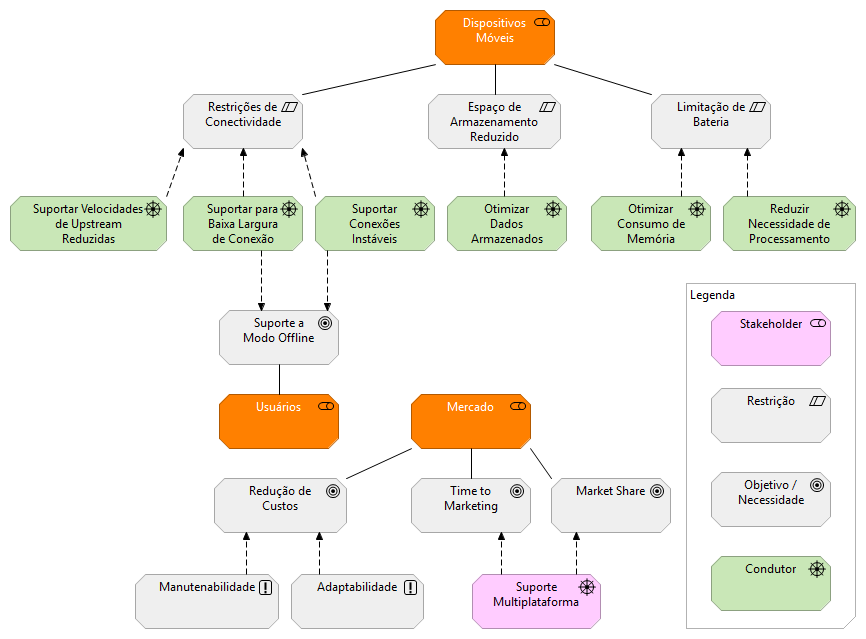
\includegraphics[scale=0.5]{images/UtilityTree}
	\caption{Árvore de Utilidade Adaptada: Stakeholders, Restrições, Objetivos, Necessidades, Condutores e suas Relações}
\end{figure}

Dispositivos móveis possuem restrições de conectividade, espaço de armazenamento reduzido e limitações de bateria.

O mercado competitivo de aplicações móveis exige redução de custos no processo de desenvolvimento o que requer manutenabilidade e adaptabilidade. Outra exigência mercadológica é por maior agilidade para lançar novos produtos ou features e ainda que os aplicativos estejam disponíveis no maior conjunto possível de plataformas dessa maneira alcançarão um volume maior de usuários em potencial.

Usuários por sua vez requerem que suas aplicações tenham suporte offline para conseguir realizar suas tarefas sobre qualquer condição de conectividade.

Considerando todos estes interesses e restrições os seguintes drivers são indispensáveis para que seja atingida uma arquitetura satisfatória:
\begin{enumerate}
	\item Suportar velocidades de upstream reduzidas.
	\item Suportar baixas larguras de conexão.
	\item Suportar instabilidade de conexão.
	\item Otimizar o volume de dados armazenados.
	\item Otimizar consumo de memória.
	\item Reduzir necessidade de processamento.
	\item Oferecer suporte multiplataforma.	
\end{enumerate}


Aplicando o método \gls{add} no passo inicial a arquitetura geral será descrita através da exposição de suas camadas mais granulares e suas responsabilidades.

\begin{figure}[H]
	\centering
	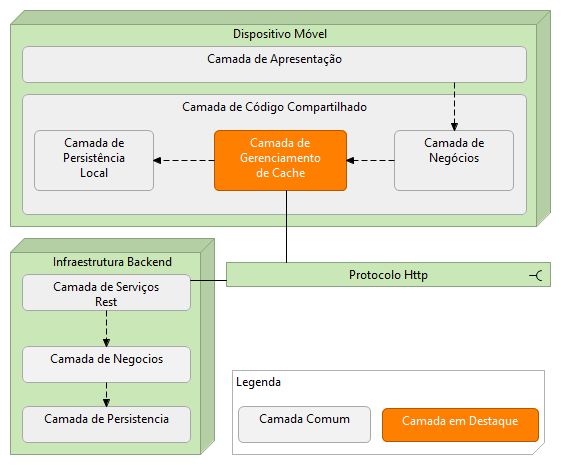
\includegraphics[scale=0.7]{images/CamadasNivel0}
	\caption{Camada de Gerenciamento de Cache e suas Interações}
\end{figure}

\begin{description}
	\item Camada de Apresentação:
	Localizada no dispositivo móvel e sua principal responsabilidade é permitir a interação entre o usuário e a aplicação.
	Numa aplicação móvel multiplataforma a camada de apresentação pode ser uniforme entre diferentes plataformas ou ser customizada para cada plataforma em que o sistema terá suporte.
	\item Camada de Código Compartilhado:
	Também localizada no dispositivo móvel constitui o coração da abordagem multiplataforma. Esta camada é responsável por agregar todos os componentes da aplicação que deverão serem compartilhados entre todas as plataformas suportadas empregando o mesmo code-base, para garantir consistência e reutilização de código.
	\begin{description}
		\item Camada de Negócios:
		Contida no dispositivo móvel é responsável por concentrar as regras de negócios da aplicação intimamente relacionadas a apresentação, incluindo formatação exibição e resposta imediata para estímulos provenientes da interação do usuário.
		\item Camada de Persistência Local: 
		Presente no dispositivo móvel é responsável realizar e gerenciar o acesso aos mecanismos de persistência local da aplicação.
		\item Camada de Gerenciamento de Cache:
		Inserida no dispositivo móvel é o segmento principal da proposição arquitetural deste trabalho. Sua atribuição é gerenciar o cache local da aplicação onde devem ser implementados todos os mecanismos de granularidade, coerência e política de substituição de cache.
	\end{description}
	\item Camada de Serviços Rest:
	Contida no \gls{back-end} é responsável por fornecer uma fachada com os serviços que podem ser consumidos pelo cliente local.
	\item Camada de Negócios:
	Também contida no \gls{back-end} é responsável por implementar todas as regras de negócio da aplicação bem como interagir com demais sistemas que fazem fronteira com a aplicação móvel, como por exemplo sistemas legados ou outros serviços internos da organização ou mesmo serviços de terceiros.
	\item Camada de persistência:
	Localizada na infraestrutura \gls{back-end} é responsável por gerenciar e implementar o armazenamento persistente dos dados da aplicação.
\end{description}

Na arquitetura proposta a Camada de Gerenciamento de Cache possui fronteira com três outras camadas possuindo um papel de destaque arquitetural por ser um elo chave entre os elementos do sistema e especialmente por conectar o segmento cliente ao segmento \gls{back-end} da aplicação.

Como sequência do desenho arquitetural o próximo elemento a ser decomposto é a Camada de Gerenciamento de Cache devido a sua aderência e decidibilidade para atendimento dos \glspl{asr} propostos.

O centro da estratégia de gerenciamento de cache é a utilização do padrão de comunicação baseado em mensagem (Message=Based Communication) \cite{meier2009microsoft} utilizando uma interface reconhecida entre todos os subelementos da Camada de Gerenciamento de Cache.

O diagrama a seguir representa as entidades utilizadas para trocar informações entre os sub-componentes desta camada:

\begin{figure}[H]
	\centering
	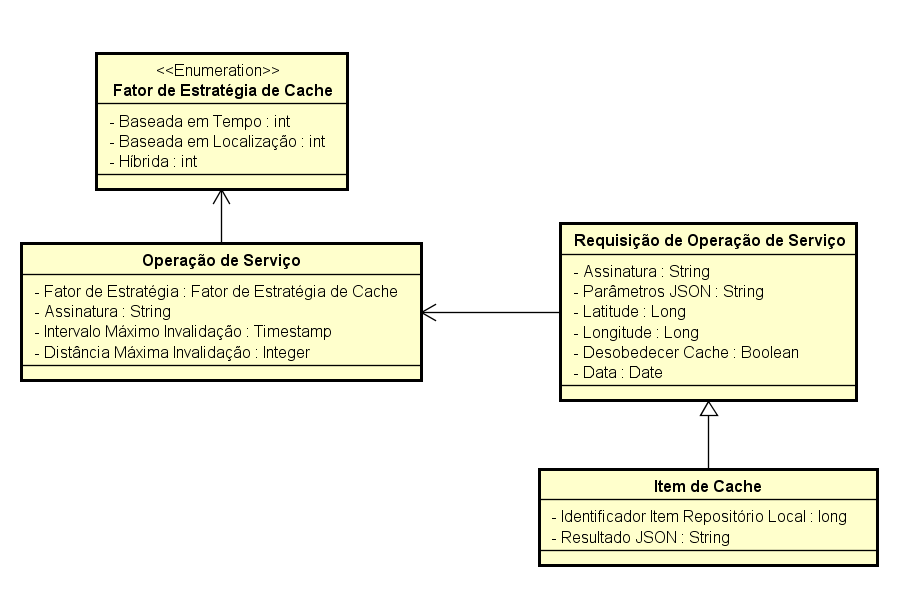
\includegraphics[scale=0.5]{images/Classes01}
	\caption{Entidades do Gerenciamento de Cache}
\end{figure}

\begin{description}
	\item Operação de Serviço:
	Representa uma operação existente na camada de serviços Rest localizada no \gls{back-end}.
	\begin{description}
		\item Fator de Estratégia: Define qual o fator de estratégia de validação está associado a operação.
		\item Assinatura: Mesma assinatura que representa o método Rest na Camada de Serviços do \gls{back-end}.
		\item Intervalo Máximo Invalidação: Período máximo para que o resultado dessa operação permaneça válido no cache levando em consideração aspectos de negócio associado a operação.
		\item Distância Máxima Invalidação: Distância/raio máximo para que o resultado dessa operação permaneça válido no cache levando em consideração aspectos de negócio associado a operação.
	\end{description}
	\item Requisição de Operação de Serviço:
	Representa uma invocação de uma operação existente na camada de serviços Rest localizada no \gls{back-end}.
	\begin{description}
		\item Assinatura: Mesma assinatura que representa o método Rest na Camada de Serviços do \gls{back-end}.
		\item Parâmetros JSON: Parâmetros de execução da operação que deverá ser executada.
		\item Latitude: Latitude do dispositivo quando a operação foi requisitada pela camada de negócios.
		\item Longitude: Longitude do dispositivo  quando a operação foi requisitada pela camada de negócios.
		\item Desobedecer Cache: Indica se esta requisição não deverá ser suprida com dados armazenados em cache.
		\item Data: Data e hora em que a operação foi requisitada pela camada de negócios.
	\end{description}
	\item Item de Cache:
	Resultado da requisição de operação de Serviço armazenada no repositório local do dispositivo. Contém todos os atributos de Requisição de Operação de Serviço e agrega atributos de identificação e resultado.
	\begin{description}
		\item Identificador Item Repositório Local: Código que identifica o item de cache no repositório local.
		\item Resultado JSON: Resultado da requisição realizada à Camada de Serviços representado no formato JSON.
	\end{description}
\end{description}

O diagrama a seguir detalha os elementos internos desta camada e como eles se relacionam com as camadas fronteiriças.

\begin{figure}[H]
	\centering
	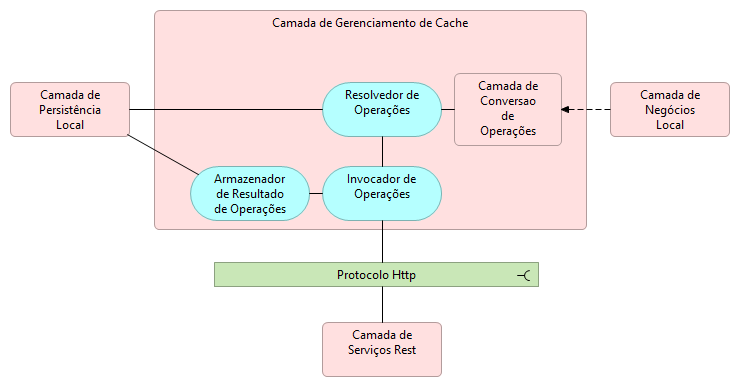
\includegraphics[scale=0.5]{images/CamadasNivel1}
	\caption{Detalhamento da Camada de Gerenciamento de Cache}
\end{figure}
 
 \begin{description}
 	\item Camada de Conversão de Operações:
 	A responsabilidade desta camada é adicionar a cada mensagem de requisição de negócio informações que sejam pertinentes ao tratamento de cache assegurando o mínimo envolvimento do código de negócio com a estratégia de cache que deverá ser adotada pela aplicação e seus mecanismos internos de funcionamento.
 	
 	Nessa camada serão definidas ocorrências das Operações de Serviço.
 	Cada requisição proveniente da camada de negócios deverá disparar uma ou mais Requisição de Operação de Serviço que serão submetidas para o componente Resolvedor de Operações.
 	
 	\item Resolvedor de Operações:
 	Este componente tem por objetivo determinar como a requisição de negócio deve ser resolvida, através de uma nova requisição a camada de serviços Rest do \gls{back-end} ou apenas consumir os dados preexistentes persistidos em repositório local para cada nova Requisição de Operação de Serviço proveniente da Camada de Conversão de Operações.
 	
 	Essa decisão será tomada com base nos seguintes critérios:
 	\begin{enumerate}
 		\item Caso a requisição não deva considerar dados em cache a resolução deverá ser concretizada diretamente através da invocação da camada de serviços no \gls{back-end}.
 		\item Caso contrário o componente deverá buscar no repositório de dados local do dispositivo um item de cache associado mesma operação utilizando os mesmos parâmetros da requisição que está sendo processada. Se nenhum resultado prévio for localizado deverá ser realizada a invocação do serviço no \gls{back-end}.
 		\item Caso seja localizado algum item de cache associado deverá ocorrer a validação se as restrições de intervalo de tempo, distância ou ambas impostas pela Operação de Serviço Associado estão sendo satisfeitas pela ocorrência disponível no repositório local.
 		Caso a validação seja positiva esta ocorrência do repositório local deverá ser retornada para a Camada de Conversão de Operações como o resultado da operação requisitada.
 		\item Caso o item de cache retornado pela consulta ao repositório local não seja validado pelas restrições da operação, este item deverá ser invalidado e deverá ser realizada uma invocação do serviço do \gls{back-end}.
 	\end{enumerate}
 	
 	\item Invocador de Operações:
 	Este componente é responsável por efetuar a invocação dos serviços Rest no BackEnd para responder às requisições de negócio e deverá ser acionado pelo Resolvedor de Operações.
 	
 	\item Armazenador de Resultado de Operações:
 	O objetivo deste componente é receber os resultados provenientes do Invocador de Operações e converte-los em um item de cache que possam ser persistidos no repositório local do dispositivo.
 	
 \end{description}

O diagrama a seguir apresenta o fluxo do processo de gerenciamento de cache proposto nesta arquitetura:

\begin{figure}[H]
	\centering
	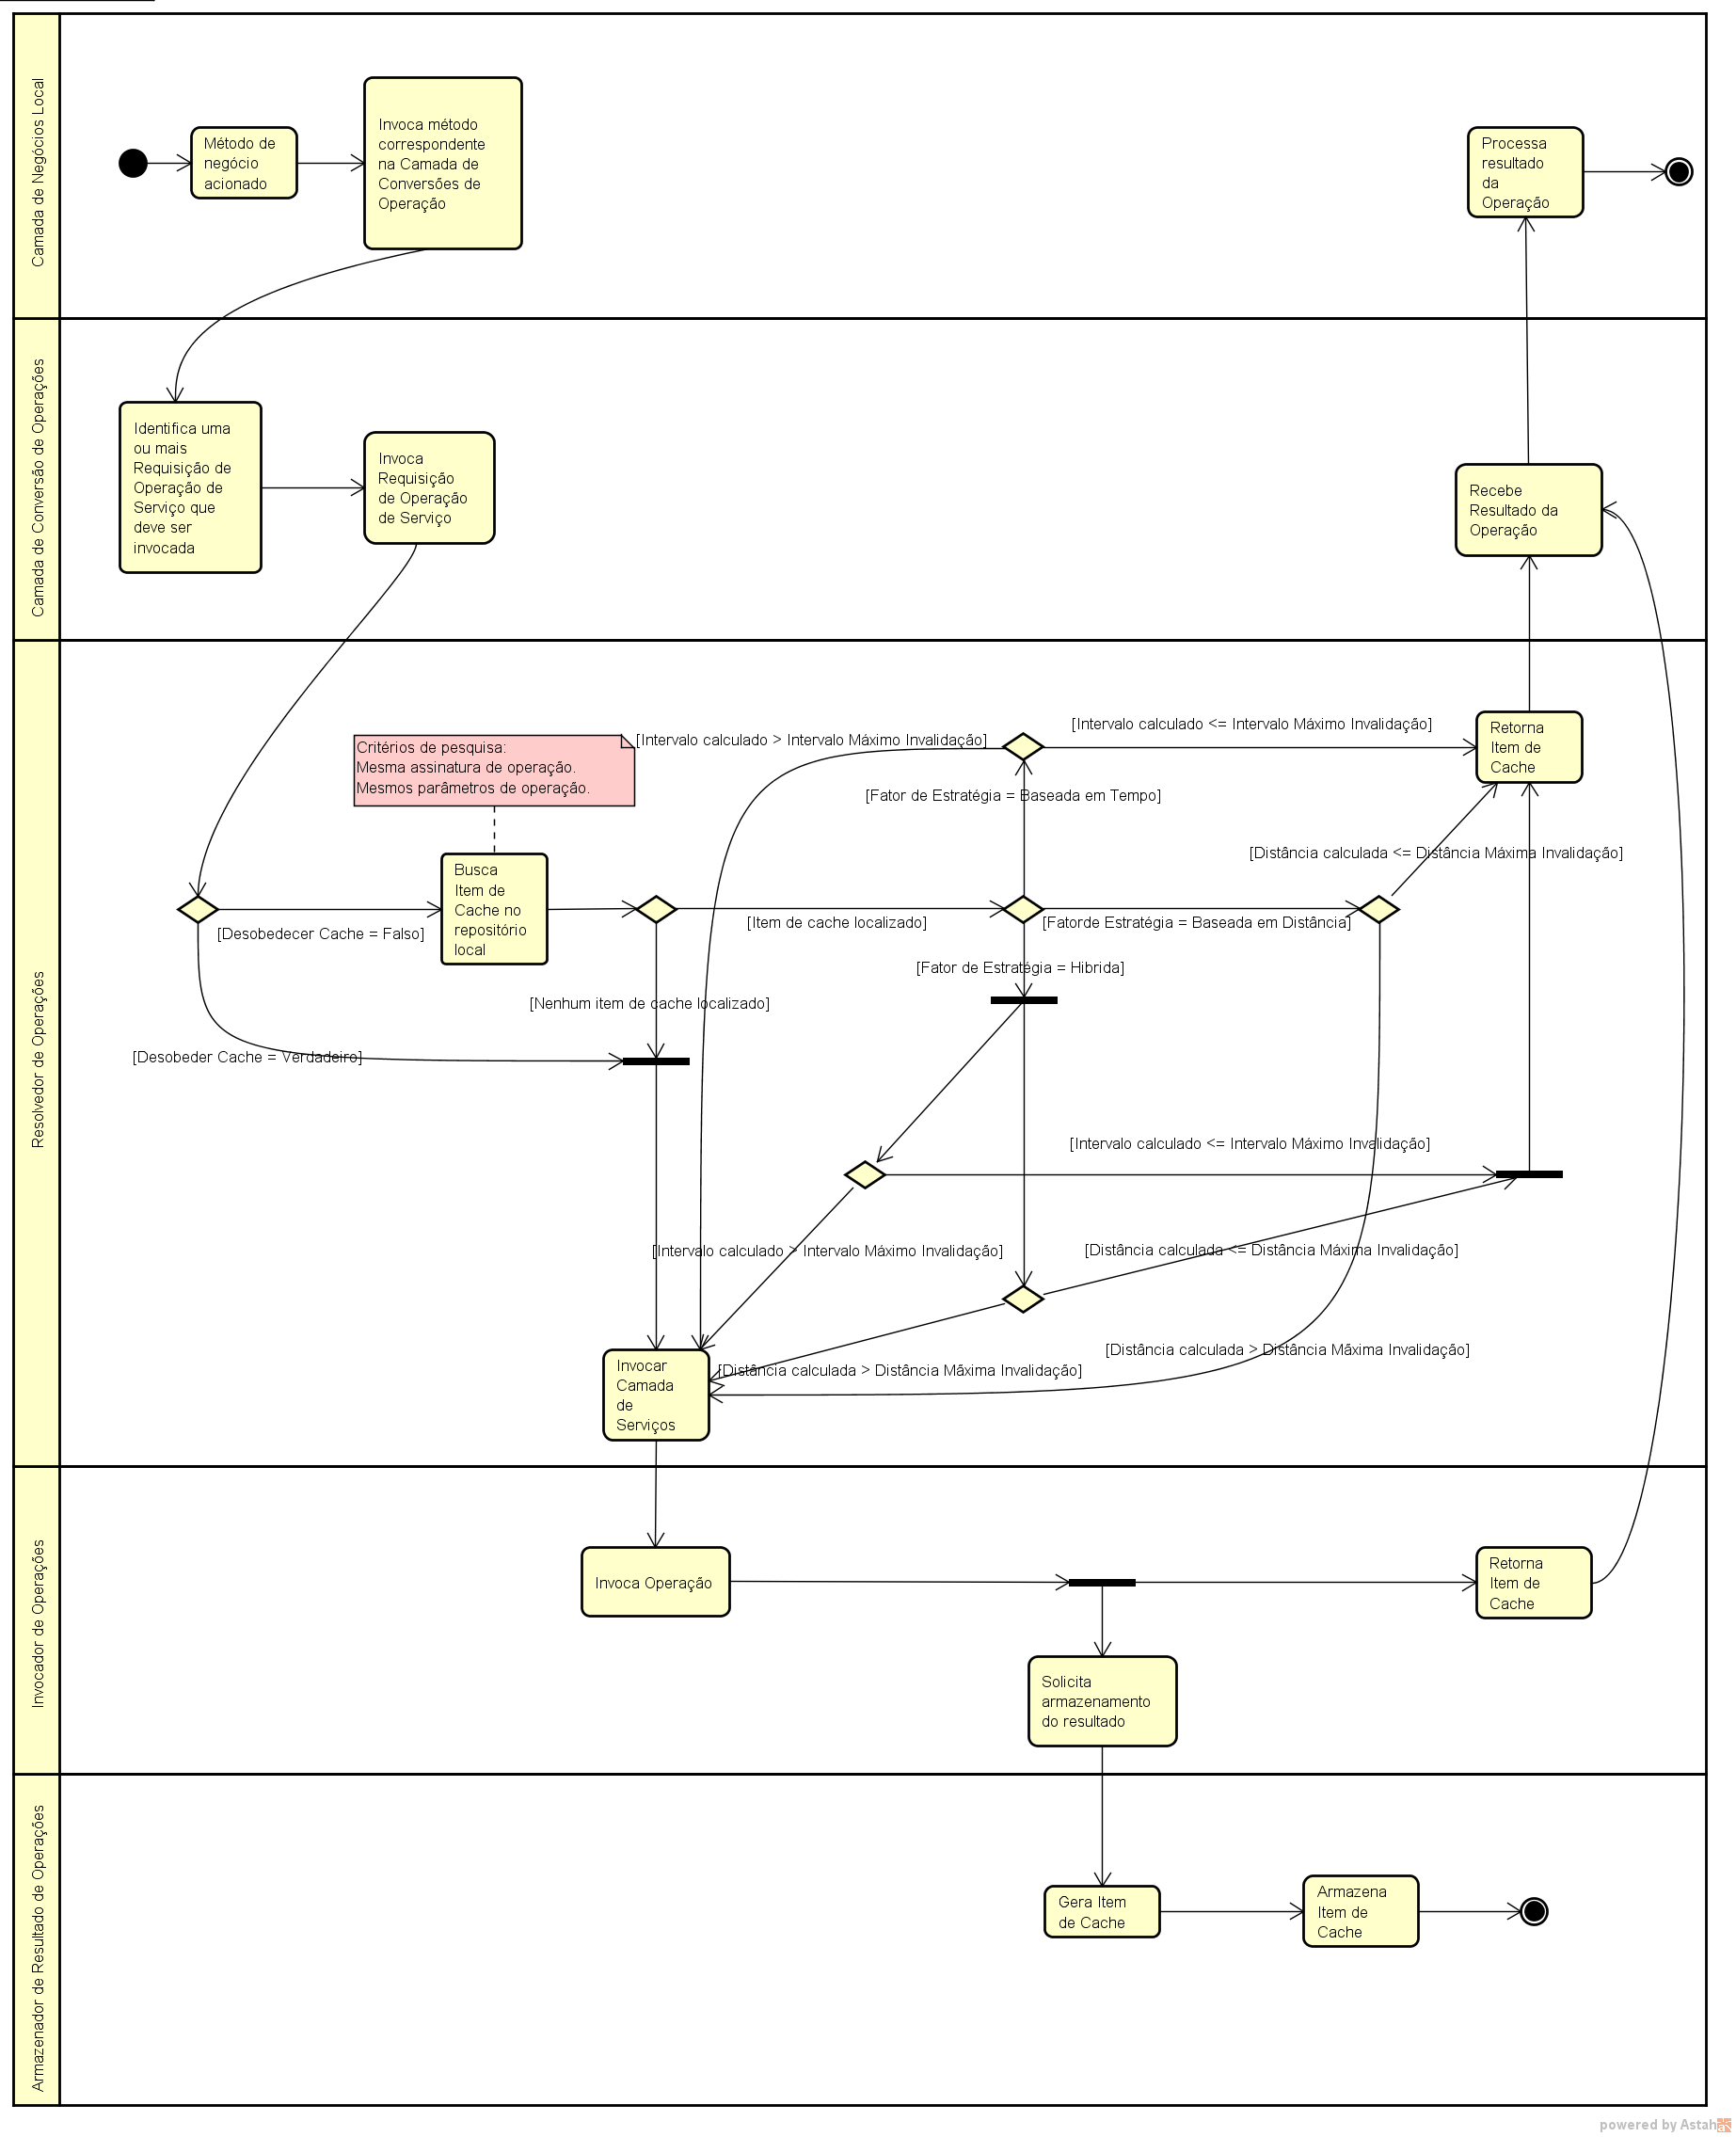
\includegraphics[scale=0.36]{images/FluxoGerenciamentodeCache}
	\caption{Fluxo Gerenciamento de Cache}
\end{figure}

\chapter{Conclusão}
A guerra pelo mercado de aplicações móveis impulsiona grandes players a disputa-lo com o lançamento de sua própria plataforma. Dessa maneira, a abordagem multiplataforma será uma realidade cada vez mais imperativa no desenvolvimento de aplicações móveis, visto que para assegurar baixo custo de desenvolvimento e cumprir o time-to-market exigido pelo mercado é necessário técnicas de engenharia de software que otimizem a produtividade e garantam coesão entre as diferentes versões de um aplicativo no processo de desenvolvimento móvel.

Coesão entre versões não implica necessariamente que a aplicação tenha exatamente o mesmo comportamento em todas as plataformas. Especialistas em usabilidade alertam sobre a importância de considerar o fator associado a fidelidade do usuário as características de sua plataforma preferida. Dessa maneira manter o look-and-feel de cada plataforma é um requisito que deve ser considerado na abordagem multiplataforma.

A arquitetura proposta endereça os objetivos deste trabalho por satisfazer a todos aos \glspl{asr} propostos para aplicações móveis multiplataforma com camada de serviços REST.

\section{Trabalhos Futuros}
\begin{enumerate}
	\item Realizar um estudo mais aprofundado sobre as categorias de aplicações móveis mais comuns em conjunto com as fábricas de software que atuem nesse ramo.
	\item Propor modelos arquiteturais que sejam aderentes as diferentes categorias de aplicações móveis para acelerar o processo de desenvolvimento.
	\item Criar templates funcionais de aplicações para permitir a rápida inicialização do desenvolvimento de aplicativos com base em seu conjunto de \glspl{asr}.
	\item Investigar o tradeoff da Descrição Arquitetural no processo de desenvolvimento de aplicações móveis, com o objetivo de estabelecer um equilíbrio entre agilidade e benefícios da documentação arquitetural.
\end{enumerate}
\bibliography{artigo}{}

% ----------------------------------------------------------
% Glossário
% ----------------------------------------------------------

% ---
% Define nome e preâmbulo do glossário
% ---
\renewcommand{\glossaryname}{Glossário}
%\renewcommand{\glossarypreamble}{Esta é a descrição do glossário.\\ \\}

% ---
% Traduções para o ambiente glossaries
% ---
\providetranslation{Glossary}{Glossário}
\providetranslation{Acronyms}{Siglas}
\providetranslation{Notation (glossaries)}{Notação}
\providetranslation{Description (glossaries)}{Descrição}
\providetranslation{Symbol (glossaries)}{Símbolo}
\providetranslation{Page List (glossaries)}{Lista de Páginas}
\providetranslation{Symbols (glossaries)}{Símbolos}
\providetranslation{Numbers (glossaries)}{Números} 
% ---

% ---
% Imprime o glossário
% ---
\cleardoublepage
\phantomsection
\addcontentsline{toc}{chapter}{\glossaryname}
% \glossarystyle{index}
% \glossarystyle{altlisthypergroup}
\glossarystyle{tree}
\printglossaries
% ---
% ---

\end{document}